\documentclass[answers]{exam}
\renewcommand{\solutiontitle}{\noindent\textbf{}\par\noindent}

\usepackage{fullpage} % Package to use full page
\usepackage{parskip} % Package to tweak paragraph skipping
\usepackage{tikz} % Package for drawing
\usepackage{amsmath}
\usepackage{blindtext}
%\usepackage{hyperref}
\usepackage{graphicx}
\usepackage{enumerate}
\usepackage{caption}
\usepackage{subcaption}
\usepackage{multicol}
\usepackage{mathptmx}
\usepackage{amsmath}
\usepackage{amssymb}
\usepackage{nameref}
\usepackage{minted}
\usepackage{graphicx}

\newcommand{\mypoints}[1]{\textcolor{red}{(#1 points)}}
\newcommand{\myinput}[1]{\textcolor{blue}{#1}}

\title{\normalfont \normalsize
\textsc{{Department of Electrical and Computer Engineering, UCLA \\
EC ENGR 188: Introduction to Computer Vision}}
\date{\vspace{-12ex}}
}
\begin{document}
\maketitle
\rule{\linewidth}{0.8pt} \\[6pt] 
\noindent
\large\textbf{\textsc{Instructor:}} Prof. Achuta Kadambi, Prof. Stefano Soatto \hfill \large\textbf{\textsc{Name:}} \myinput{Anuj Agrawal}\\
\large\textbf{\textsc{TA:}} Zhen Wang \hfill 
\large\textbf{\textsc{UID:}} \myinput{605627630}
\rule{\linewidth}{0.8pt} \\[6pt] 

\begin{center}
{\textsc{Homework 2}} 
\end{center}
% \vspace{2cm}


\begin{table}[h]
\centering
\resizebox{0.8\textwidth}{!}{%
\begin{tabular}{cccc}
\hline
\multicolumn{1}{c}{\textsc{Problem}} &
\multicolumn{1}{c}{\textsc{Type}} &
\multicolumn{1}{c}{\textsc{Topic}} & \multicolumn{1}{c}{\textsc{Max. Points}} \\  \hline \\ 
 1 & Analytical & Filter Design &  10 \\ [2mm]
 2 & Analytical + Coding & Blob Detection &  10 \\ [2mm]
 3 & Coding & Corner Detection &  10 \\ [2mm]
 4 & Analytical & 2D Transformation &  10 \\ [2mm]
 5 & Analytical & Interview Question & 5 \\ [2mm]
\hline
\end{tabular}
}
\caption*{}
\label{}
\end{table}

\newpage

\section*{Motivation}

In the previous homework, we have seen how to process images using convolutions and mine images for features such as edges using image gradients. In this homework, we will detect other types of useful features in images such as blobs and corners that can be useful for a variety of computer vision tasks. We then transition from detecting useful features in images to relating different images via 2D transformations.

The problem set consists of: 
\begin{itemize}
    \item analytical questions to solidify the concepts covered in the class; and
    \item coding questions to implement some of the algorithms described in class using Python.
\end{itemize}

\section*{Homework Layout}
The homework consists of 5 problems in total, with subparts for each problem. There are 2 types of problems in this homework - analytical and coding. We encourage you to answer all the problems using the Overleaf document; however, handwritten solutions will also be accepted. 

\section*{Submission}

You will need to make two submissions: (1) Gradescope: You will submit a PDF with all the answers on Gradescope. (2) CCLE: You will submit your Jupyter notebook (.ipynb file) with filename $\{$your UID$\}$.ipynb with all the cells executed on CCLE. 


\newpage
\section{Filter Design \mypoints{10.0}}
In the class you were taught the Central Difference/Laplacian filter for detecting the edges in an image (by computing the gradients along the horizontal and vertical directions). In the discussion we derived those filters by approximating the first (for gradient) and second derivative (for Laplacian) of a univariate function $f(x)$ using the Taylor series expansion of $f(x+h)$ and $f(x-h)$, where $h$ is a small perturbation around $x$ with $h=1$ for the discrete case. These filters only consider the adjacent neighbours of the current pixel. In this question you will derive a high-order approximation for the two filters, such that the filters will use 2 adjacent neighbours. To summarize, you will be deriving a higher order approximation to the first/second derivative of $f(x)$. We will use $f^{(1)}(x),f^{(2)}(x)$ to denote the first and second derivative respectively.

\subsection{Compute $f(x+h)$ \mypoints{1.0}}
Write the Taylor series approximation for $f(x+h)$ around $f(x)$, such that the approximation error tends to 0 as $h^5$, i.e. consider only the first 5 terms in the Taylor series approximation. Use $f^{(1)}(x)$ for the first derivative, $f^{(2)}(x)$ for the second derivative and so on. 
\begin{solution}
$f(x+h) = f(x) + \dfrac{f^{(1)}(x)(h)}{1!} + \dfrac{f^{(2)}(x)(h)^2}{2!}+ \dfrac{f^{(3)}(x)(h)^3}{3!}+ \dfrac{f^{(4)}(x)(h)^4}{4!}$
\end{solution}

\subsection{Compute $f(x-h)$ \mypoints{1.0}}
Similarly, write the Taylor series approximation for $f(x-h)$ around $f(x)$, such that the approximation error tends to 0 as $h^5$.
\begin{solution}
$f(x-h) = f(x) - \dfrac{f^{(1)}(x)(h)}{1!} + \dfrac{f^{(2)}(x)(h)^2}{2!} - \dfrac{f^{(3)}(x)(h)^3}{3!}+ \dfrac{f^{(4)}(x)(h)^4}{4!}$
\end{solution}

\subsection{Compute $f(x+h)-f(x-h)$ \mypoints{1.0}}
\label{difference}
Using the expressions you obtained in the previous two parts, compute the expression for $f(x+h)-f(x-h)$. You may assume that $\mathcal{O}(h^5)$ tends to 0, so that you can neglect the term. You will be using this result to compute a high-order approximation to $f^{1}(x)$.
\begin{solution}
$f(x+h) - f(x-h) =  \dfrac{2f^{(1)}(x)(h)}{1!} + \dfrac{2f^{(3)}(x)(h)^3}{3!}$
\end{solution}

\subsection{Unknowns at each pixel \mypoints{1.0}}
\label{unknowns}
Let's assume that you have access to $f(x)$, which is a 1D signal (or equivalently one row in an image). This means that you can easily obtain the values for $f(x)$, $f(x \pm h)$, $f(x \pm 2h)$ and so on (assuming appropriate zero padding for start and end values). However, for each pixel $x$, if you only consider using its adjacent neighbours ($\pm h$), then the equation in the previous part has 2 unknowns. What are the two unknowns?
\textit{Note:} $h=1$ for the discrete case, so $h$ is not an unknown. But don't substitute $h=1$ as of now; we will substitute it later.
\begin{solution}
The two unknowns are:
\begin{enumerate}
  \item $f^{(1)}(x)$
  \item $f^{(3)}(x)$
\end{enumerate}
\end{solution}

\subsection{Compute $f^{(1)}(x)$ \mypoints{1.0}}
\label{gradient}
From the previous part, you know that for each pixel $x$, if we only consider $x \pm h$, then we have 1 equation and 2 variables (underdetermined system). To mitigate this issue, we consider two adjacent neighbours for each pixel ($x \pm 2h$) in addition to $x \pm h$. Replace $h$ with $2h$ in the previous equation and you will get another equation for that pixel. So now, for each pixel, you have 2 equations and 2 variables. One equation should have $f(x \pm h)$ and the other should have $f(x \pm 2h)$. Using these two equations, solve for $f^{(1)}(x)$.
\begin{solution}
\begin{align}
f(x+h) - f(x-h) =  \dfrac{2f^{(1)}(x)(h)}{1!} + \dfrac{2f^{(3)}(x)(h)^3}{3!}\\
f(x+2h) - f(x-2h) =  \dfrac{2f^{(1)}(x)(2h)}{1!} + \dfrac{2f^{(3)}(x)(2h)^3}{3!}
\end{align} 

Multiplying equation (1) with 8 gives 
\begin{align}
8f(x+h) - 8f(x-h) =  \dfrac{16f^{(1)}(x)(h)}{1!} + \dfrac{16f^{(3)}(x)(h)^3}{3!}
\end{align} 
Subtracting equation (2) from (3) gives
\begin{align}
8f(x+h) - 8f(x-h) - f(x+2h) + f(x-2h)=  \dfrac{12f^{(1)}(x)(h)}{1!}\\
f^{(1)}(x) = \dfrac{8f(x+h) - 8f(x-h) - f(x+2h) + f(x-2h)}{12h}
\end{align} 

\end{solution}

\subsection{Convolution Kernel \mypoints{1.0}}
What is the convolution kernel corresponding to the new filter for $f^{(1)}(x)$? Substitute $h=1$ for the discrete case. This filter is now a higher order central-difference filter which can be used to compute the gradients/edges.
\begin{solution}
Convolution kernel of $f^{(1)}(x)$ :
$[+1, -8, 0, 8, -1]/12$
\end{solution}

\subsection{Laplacian Filter \mypoints{1.0}}
We will repeat the same exercise as the previous parts; however, now we compute a higher order approximation to the Laplacian filter. Similar to \ref{difference}, compute the expression for $f(x+h) + f(x-h)$.
\begin{solution}
$f(x+h) + f(x-h) = 2f(x) + \dfrac{2f^{(2)}(x)(h)^2}{2!} + \dfrac{2f^{(4)}(x)(h)^4}{4!}$
\end{solution}

\subsection{Unknowns for the Laplacian \mypoints{1.0}}
Similar to \ref{unknowns}, what are the two unknowns for each pixel in the expression from the previous part?
\begin{solution}
The two unknowns are:
\begin{enumerate}
  \item $f^{(2)}(x)$
  \item $f^{(4)}(x)$
\end{enumerate}
\end{solution}

\subsection{Compute $f^{(2)}(x)$ \mypoints{1.0}}
Similar  to \ref{gradient}, use $f(x \pm 2h)$ to solve for $f^{(2)}(x)$. Write the expression for $f^{(2)}(x)$.
\begin{solution}
\begin{align}
f(x+h) + f(x-h) = 2f(x) + \dfrac{2f^{(2)}(x)(h)^2}{2!} + \dfrac{2f^{(4)}(x)(h)^4}{4!}\\
f(x+2h) + f(x-2h) = 2f(x) + \dfrac{2f^{(2)}(x)(2h)^2}{2!} + \dfrac{2f^{(4)}(x)(2h)^4}{4!}
\end{align} 

Multiplying equation (6) with 16 gives 
\begin{align}
16f(x+h) + 16f(x-h) = 32f(x) + \dfrac{32f^{(2)}(x)(h)^2}{2!} + \dfrac{32f^{(4)}(x)(h)^4}{4!}
\end{align} 
Subtracting equation (7) from (8) gives
\begin{align}
16f(x+h) + 16f(x-h) - f(x+2h) - f(x-2h)= 30f(x) + \dfrac{24f^{(2)}(x)(h^2)}{2!}\\
f^{(2)}(x) = \dfrac{16f(x+h) + 16f(x-h) - f(x+2h) - f(x-2h) - 30f(x)}{12h^2}
\end{align} 
\end{solution}

\subsection{Convolution Kernel \mypoints{1.0}}
What is the corresponding convolution for the filter you derived in the previous part? Use $h=1$ for the discrete case.
\begin{solution}
Convolution kernel of $f^{(2)}(x)$ :
$[-1, +16, -30, +16, -1]/12$
\end{solution}

\newpage
\section{Blob Detection \mypoints{10.0}}
In this question, you will be using the Laplacian of Gaussian (LoG) filter to detect blobs in an image. Let's consider a 2D Gaussian $G_{\sigma}(x,y) = \dfrac{1}{2\pi \sigma^2} e^{-\big(\dfrac{x^2+y^2}{2\sigma^2}\big)}$. Remember that we need to smooth the image using a Gaussian filter before computing the Laplacian to prevent noise amplification. However, instead of computing the Laplacian after filtering the image with a Gaussian kernel, we can directly filter the image with the Laplacian of Gaussian filter.

\subsection{Compute $\dfrac{\partial^2G_{\sigma}(x,y)}{\partial x^2}$ \mypoints{1.0}}
Write the expression for $\dfrac{\partial ^2G_{\sigma}(x,y)}{\partial x^2}$.
\begin{solution}
$\dfrac{\partial^2G_{\sigma}(x,y)}{\partial x^2} = \dfrac{1}{2\pi \sigma^4}\big(\dfrac{x^2}{\sigma^2} -1\big) e^{-\big(\dfrac{x^2+y^2}{2\sigma^2}\big)}$
\end{solution}

\subsection{Compute $\dfrac{\partial^2G_{\sigma}(x,y)}{\partial y^2}$ \mypoints{1.0}}
Write the expression for $\dfrac{\partial^2G_{\sigma}(x,y)}{\partial y^2}$.
\begin{solution}
$\dfrac{\partial^2G_{\sigma}(x,y)}{\partial y^2} = \dfrac{1}{2\pi \sigma^4}\big(\dfrac{y^2}{\sigma^2} -1\big) e^{-\big(\dfrac{x^2+y^2}{2\sigma^2}\big)}$
\end{solution}

\subsection{Laplacian of a 2D Gaussian \mypoints{1.0}}
Using the results from the previous parts, write the expression for the Laplacian of a 2D Gaussian, $L(x,y)$.
\begin{solution}
$L(x,y) = -\dfrac{1}{\pi \sigma^4}\big(1 - \dfrac{x^2 + y^2}{2\sigma^2}\big) e^{-\big(\dfrac{x^2+y^2}{2\sigma^2}\big)} $
\end{solution}

\subsection{Scale-Normalization \mypoints{1.0}}
In class, we studied that it is important to normalize the scale of $L(x,y)$ before using it for blob detection. What is the normalization factor? Provide justification.
\begin{solution}
Scale normalized LOG(x,y): $\sigma^2 L(x,y) = -\dfrac{1}{\pi \sigma^2}\big(1 - \dfrac{x^2 + y^2}{2\sigma^2}\big) e^{-\big(\dfrac{x^2+y^2}{2\sigma^2}\big)} $\\

The magnitude of LoG filter achieves a maximum at the center of a scale matched blob. As we increase sigma, the image pixel intensity decreases and image derivatives are exponentially attenuated. Without normalization the maximum is at the finest scale and the minimum is at the coarsest scale. To keep the response scale-invariant we need to normalize the response by multiplying the n-th derivative by $\sigma^n$. Since the LoG is second derivatives, we multiply it by $\sigma^2$. 

\end{solution}

\subsection{LoG Filter \mypoints{1.0}}
(See the Jupyter notebook) Using the expression for $L(x,y)$ and the scale normalization, write a Python function which will compute the LoG Filter.
\begin{solution}
% \vspace{2cm} % remove this
\begin{minted}{python}
def log_filter(size: int, sigma: float):
  kernel = np.zeros((size,size))
  for i in range(size):
    for j in range(size):
      x = i - size//2
      y = j - size//2
      kernel[i,j] =-1*(1-(x**2 + y**2)/(2*(sigma**2)))*\
      np.exp(-(x**2 + y**2)/(2*(sigma**2)))/(np.pi*(sigma**2))
  return kernel
\end{minted}
\end{solution}

\subsection{$\sigma$ values \mypoints{1.0}}
(See the Jupyter notebook) What are the 5 sigma values which give the maximum response? To visualize the response, you can use the colormap in the Jupyter notebook.
\begin{solution}
For a binary circle with radius r, the value of sigma at which the laplacian reaches a maxima is given by:\\
$$\sigma(r) = \frac{r}{\sqrt{2}}$$\\
$\sigma(5) = \frac{5}{\sqrt{2}} = 3.53$\\
$\sigma(10) = \frac{10}{\sqrt{2}} = 7.07$\\
$\sigma(15) = \frac{15}{\sqrt{2}} = 10.60$\\
$\sigma(20) = \frac{20}{\sqrt{2}} = 14.14$\\
$\sigma(35) = \frac{35}{\sqrt{2}} = 24.75$\\
(approximated to 2 decimal places)
\end{solution}

\subsection{Visualize LoG Filter \mypoints{1.0}}
(See the Jupyter notebook) In this sub-part you will visualize the LoG filter. Copy the saved image from the Jupyter notebook here. 
\begin{solution}
% \vspace{2cm} % remove this
\begin{figure}[H]
    \centering
    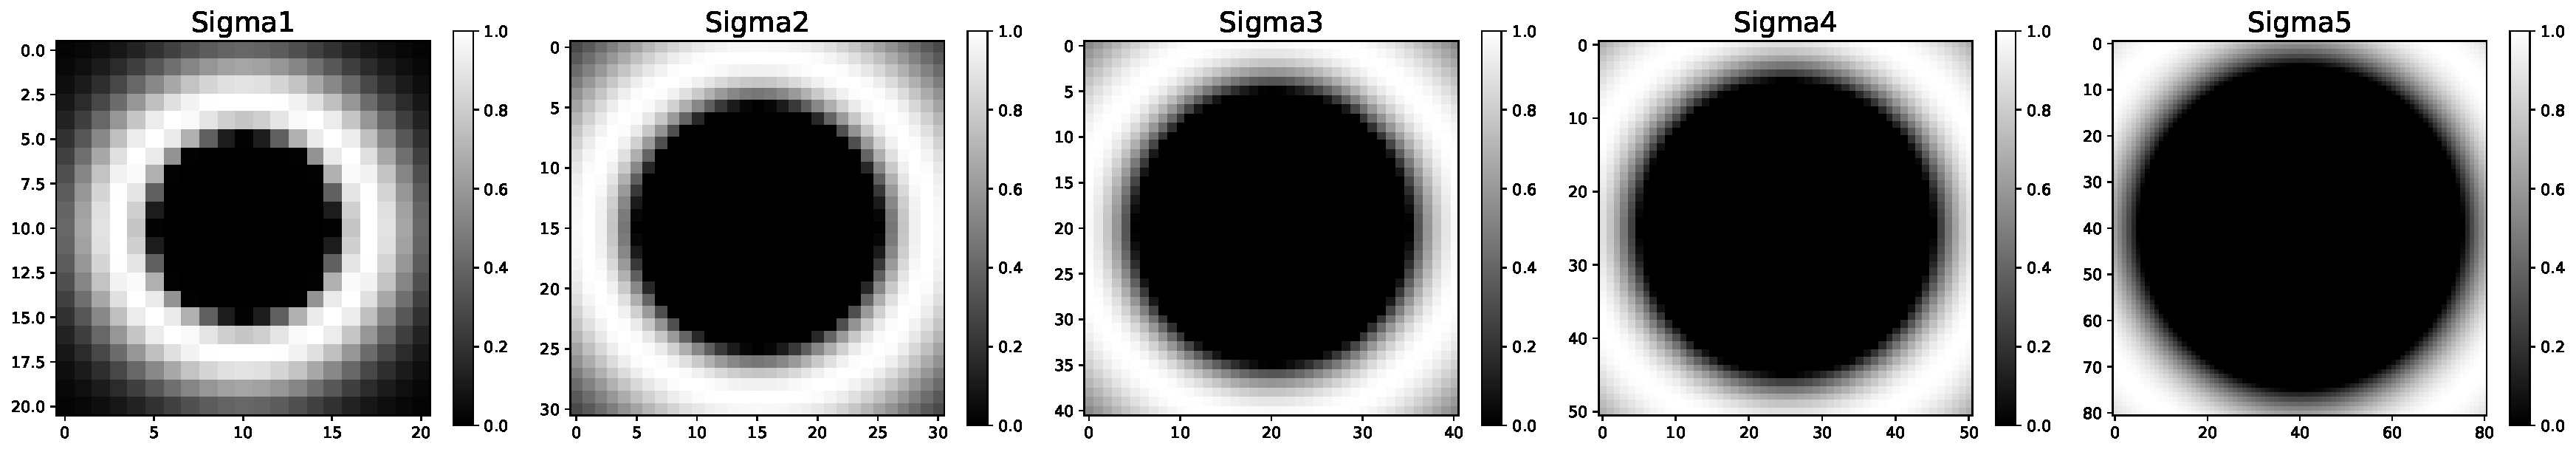
\includegraphics[width=1.0\linewidth]{Images/question_2_7.pdf}
\end{figure}
\end{solution}

\subsection{Visualize the blob detection results \mypoints{3.0}}
(See the Jupyter notebook) In this sub-part you will visualize the blob detection results. Copy the saved image from the Jupyter notebook here. 
\begin{solution}
% \vspace{2cm} % remove this
\begin{figure}[H]
    \centering
    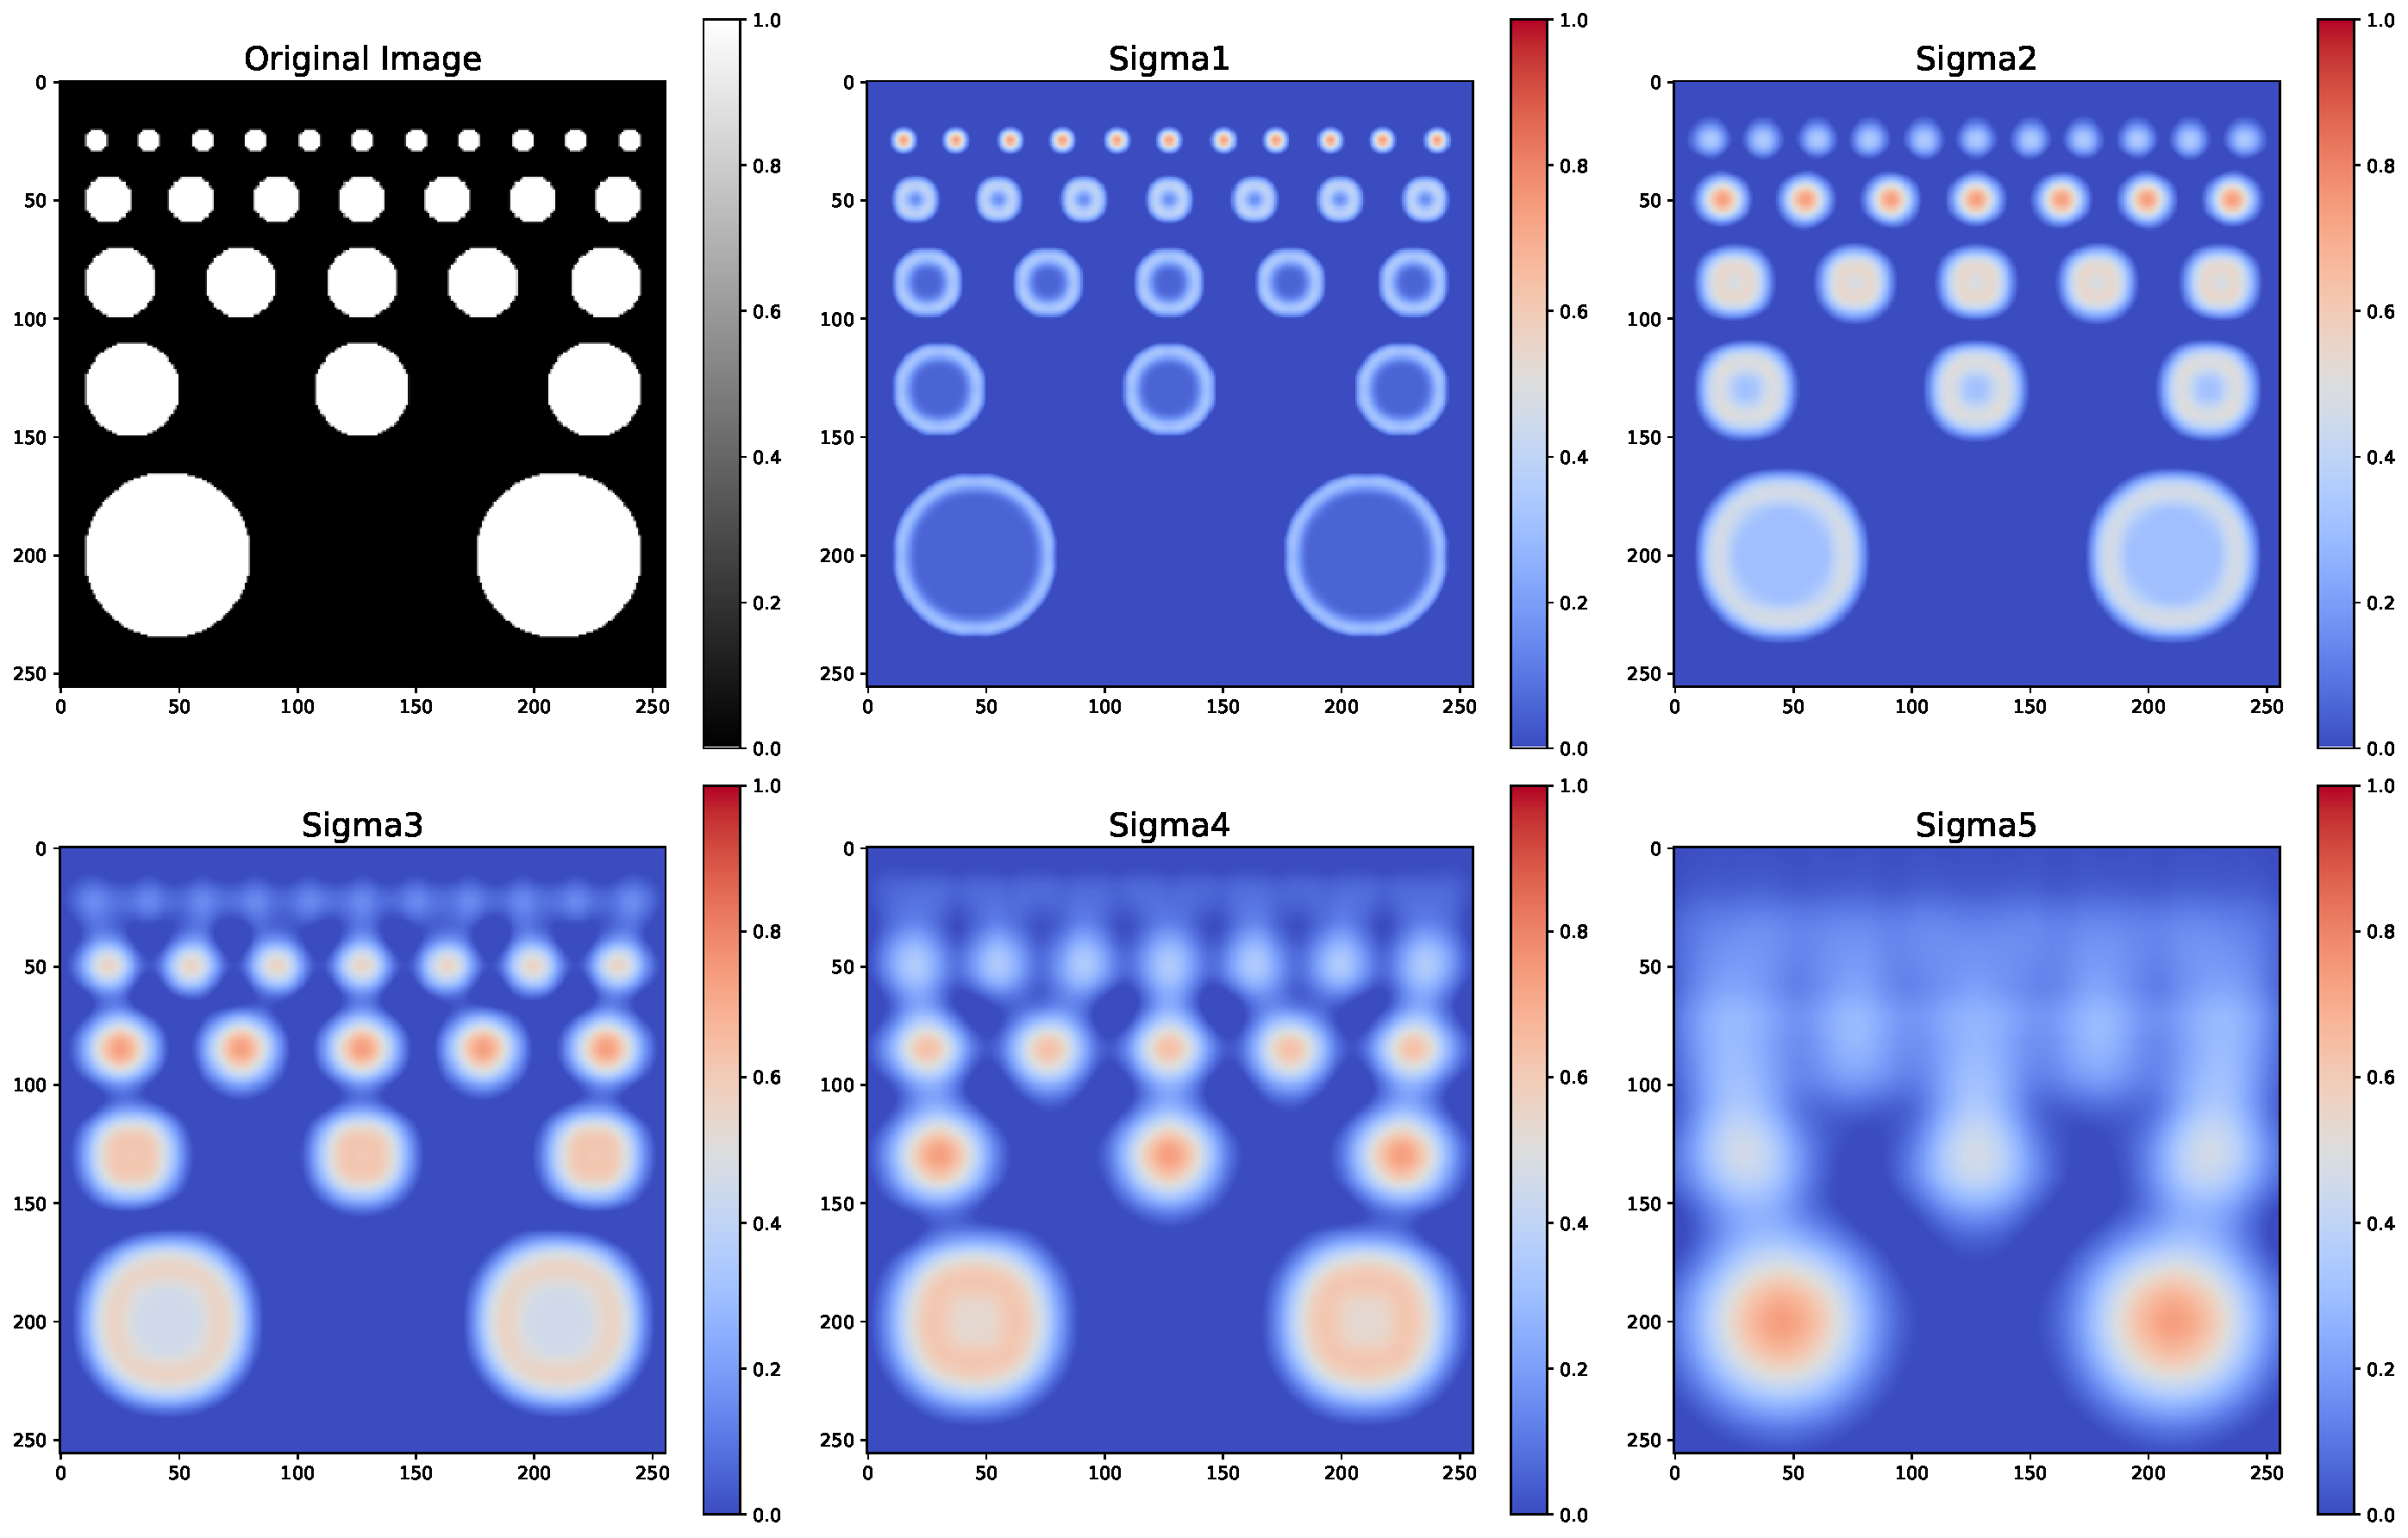
\includegraphics[width=1.0\linewidth]{Images/question_2_8.pdf}
\end{figure}
\end{solution}

\newpage
\section{Corner Detection \mypoints{10.0}}

In this question, you will be implementing the Harris corner detector. As discussed in class, corners generally serve as useful features.

\subsection{Computing Image Gradients Using Sobel Filter \mypoints{1.0}}
(See the Jupyter notebook). In this sub-part, you will write a function that computes image gradients using the Sobel filter. Make sure that your code is within the bounding box.

\begin{solution}
% \vspace{2cm} % remove this
\begin{minted}{python}
def compute_image_gradient(image: np.array):
  return conv2D(image, sobel_x), conv2D(image, sobel_y)
\end{minted}
\end{solution}

\subsection{Visualizing the Image Gradients \mypoints{1.0}}
(See the Jupyter notebook). In this sub-part, you will visualize the image gradients. Copy the saved image from the Jupyter notebook here.

\begin{solution}
% \vspace{2cm} % remove this
\begin{figure}[H]
    \centering
    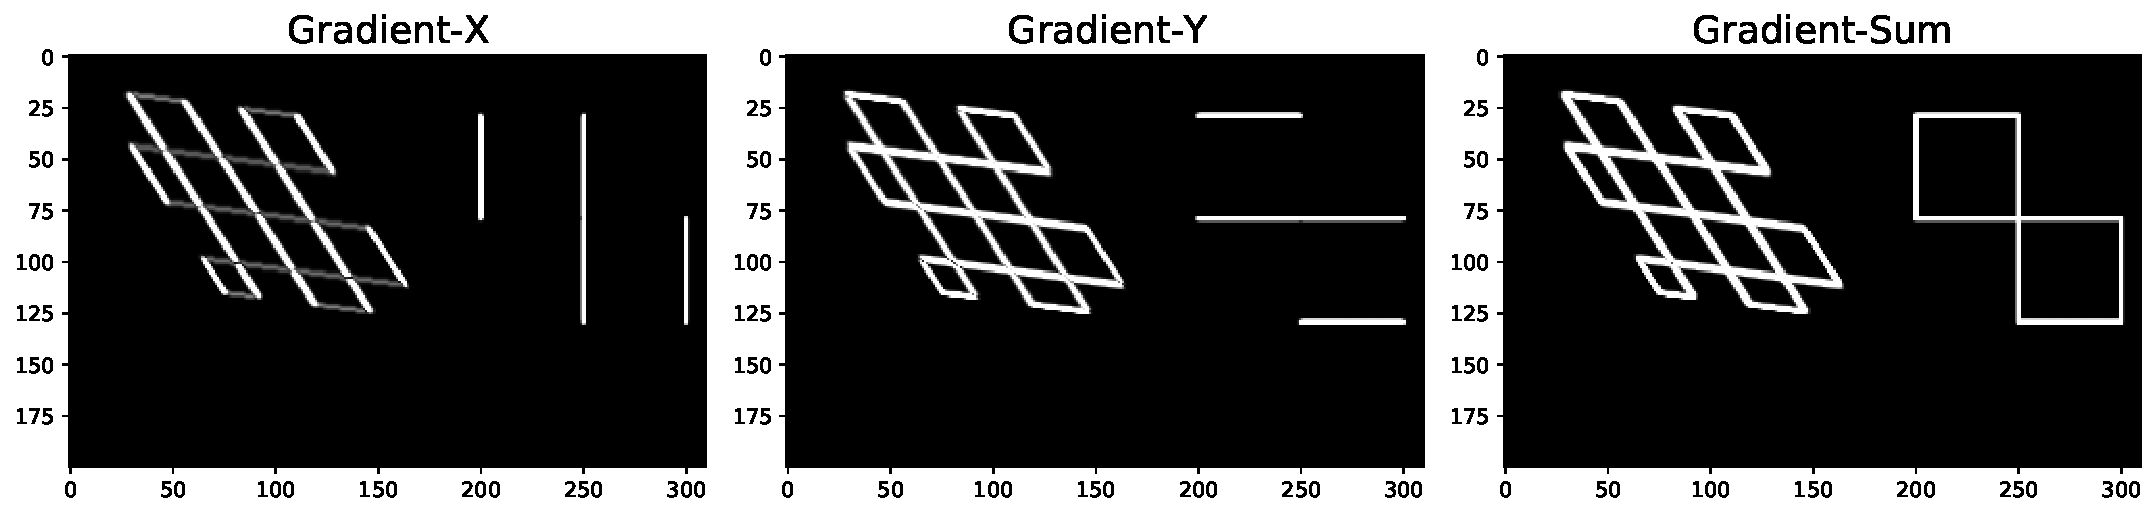
\includegraphics[width=\linewidth]{Images/question_3_2.pdf}
\end{figure}
\end{solution}

\subsection{Computing the Covariance Matrix \mypoints{1.0}}
(See the Jupyter notebook). In this sub-part, you will write a function that computes the covariance matrix of the image gradients. Make sure that your code is within the bounding box.

\begin{solution}
% \vspace{2cm} % remove this
\begin{minted}[breaklines]{python}
def grad_covariance(image: np.array, size: int):
  img_gradient_x, img_gradient_y = compute_image_gradient(image)
  mean = average_filter(size)
  Ixx = img_gradient_x * img_gradient_x
  Ixy = img_gradient_x * img_gradient_y
  Iyy = img_gradient_y * img_gradient_y

  Ixx = conv2D(Ixx, mean) * (size**2)
  Ixy = conv2D(Ixy, mean) * (size**2)
  Iyy = conv2D(Iyy, mean) * (size**2)
  
  return Ixx, Ixy, Iyy
\end{minted}
\end{solution}

\subsection{Harris Corner Response \mypoints{1.0}}
(See the Jupyter notebook). In this sub-part, you will write a function that computes the Harris response function. Make sure that your code is within the bounding box.

\begin{solution}
% \vspace{2cm} % remove this
\begin{minted}[breaklines]{python}
def harris_response(image: np.array, k: float, size: int):
  Ixx, Ixy, Iyy  = grad_covariance(image, size)
  trace = Ixx + Iyy #Trace
  det = (Ixx * Iyy) - (Ixy**2) #Determinant
  R = det - k * trace**2 #Response
  return R
\end{minted}
\end{solution}

\subsection{Visualizing the Harris Corner Detector \mypoints{1.0}}
(See the Jupyter notebook). In this sub-part, you will visualize the Harris corner detections. Copy the saved image from the Jupyter notebook here.

\begin{solution}
% \vspace{2cm} % remove this
\begin{figure}[H]
    \centering
    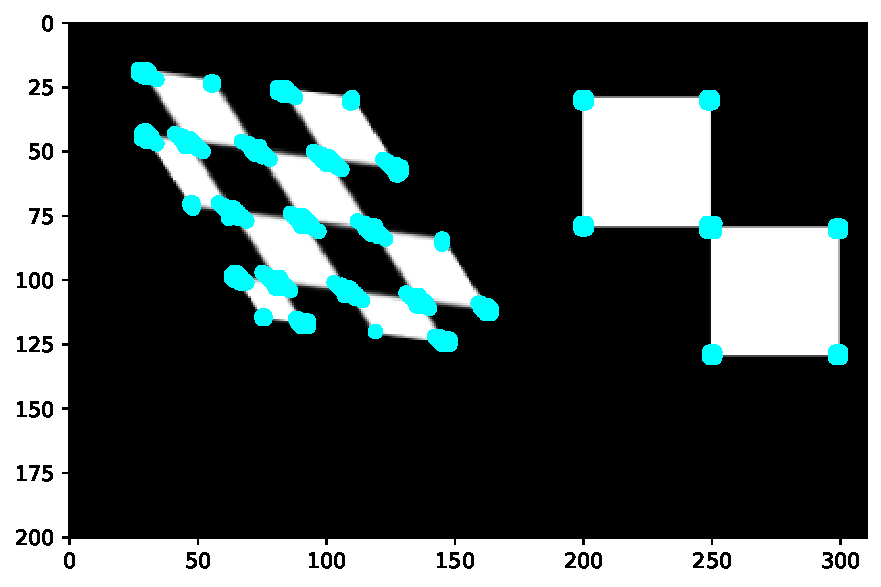
\includegraphics[width=\linewidth]{Images/question_3_5.pdf}
\end{figure}
\end{solution}

\subsection{Thresholding the Harris Response \mypoints{1.0}}
To remove duplicate detections, you will write a function that applies non-maximum suppression to the Harris corner detections. To make writing this function easier, you will implement it in various parts.

(See the Jupyter notebook). In this sub-part, you will implement the first step of non-maximum suppression: thresholding the Harris response to obtain candidate corner detections. Make sure that your code is within the bounding box.

\begin{solution}
% \vspace{2cm} % remove this
\begin{minted}[breaklines]{python}
def threshold_harris_response(harris_response: np.array, threshold: float):
  coords = np.argwhere(harris_response > threshold)
  return coords
  
\end{minted}
\end{solution}

\subsection{Sorting Candidate Detections \mypoints{1.0}}
(See the Jupyter notebook). In this sub-part, you will sort the candidate detections by maximum Harris response value. Make sure that your code is within the bounding box.

\begin{solution}
% \vspace{2cm} % remove this
\begin{minted}[breaklines]{python}
def sort_detections(candidate_detections: np.array, harris_response: np.array):
  coords_list = candidate_detections.tolist()
  
  for i in range(len(coords_list)-1):
    if (harris_response[coords_list[i][0]][coords_list[i][1]])\
     < harris_response[coords_list[i+1][0]][coords_list[i+1][1]]:
      coords_list[i], coords_list[i+1] = coords_list[i+1], coords_list[i] #swap

  candidate_detections_sorted = np.asarray(coords_list)
  return candidate_detections_sorted 
\end{minted}
\end{solution}

\subsection{Suppressing Non-max Detections \mypoints{1.0}}
(See the Jupyter notebook). In this sub-part, you will implement the final step of non-maximum suppression: removing corner detections that are not local maxima. Make sure that your code is within the bounding box.

\begin{solution}
% \vspace{2cm} % remove this
\begin{minted}[breaklines]{python}
def local_max(sorted_detections: np.array, distance: float):
  max_arr = np.array([sorted_detections[0]])
  for p1 in range(1, len(sorted_detections)):
    ele_p1 = sorted_detections[p1]
    flag = True
    for p2 in range(p1):
      ele_p2 = sorted_detections[p2]
      if (l2_distance(ele_p1, ele_p2) <= distance): 
        flag = False
        break
    if flag : max_arr = np.append(max_arr, [ele_p1], axis = 0)

  return max_arr
  
\end{minted}
\end{solution}

\subsection{Non-Maximum Suppression: Putting it all together \mypoints{1.0}}
(See the Jupyter notebook). In this sub-part, you will write a function that performs non-maximum suppression on the Harris corner response. Make sure that your code is within the bounding box.

\begin{solution}
% \vspace{2cm} % remove this
\begin{minted}[breaklines]{python}
def non_max_suppression(harris_response: np.array, distance: float, threshold: float):

  candidate_detections =  threshold_harris_response(harris_response, threshold)
  sorted_detections = sort_detections(candidate_detections, harris_response)
  max_elements = local_max(sorted_detections, distance)
  return max_elements
\end{minted}
\end{solution}


\subsection{Visualizing Harris Corner Detections + Non-maximum Suppression \mypoints{1.0}}
(See the Jupyter notebook). In this sub-part, you will visualize the Harris corner detections after non-maximum suppression has been applied. Copy the saved image from the Jupyter notebook here. Duplicate corner detections should now be removed.

\begin{solution}
% \vspace{2cm} % remove this
\begin{figure}[H]
    \centering
    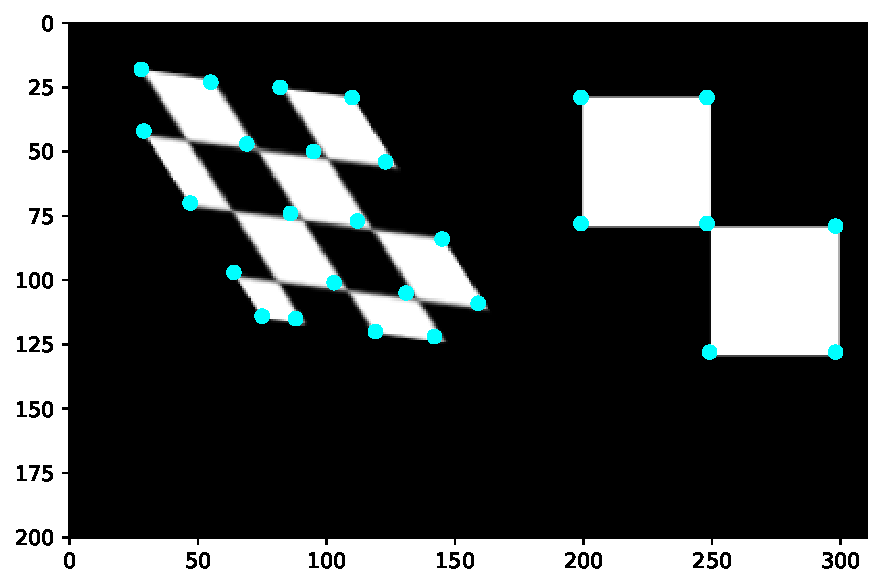
\includegraphics[width=\linewidth]{Images/question_3_10.pdf}
\end{figure}
\end{solution}

\newpage
\section{2D Transformation \mypoints{10.0}}
In this question, you will be identifying different 2D transformations. You will be given a set of feature points $x$ and the corresponding transformed points $x'$. Given these two set of points, you have to identify the 2D transformation. For the first 5 sub-parts, there is only one transformation (translation, scaling, rotation, shearing). For the next parts, there may be more than one transformation.
While justifying your answer for each part you should also write the $3 \times 3$ transformation matrix $M$.

\subsection{Example 1 \mypoints{1.0}}
$x = \{(1,1), (2,1), (2,2), (1,2)\}$ and $x' = \{(2,2), (3,2), (3,3), (2,3)\}$. Identify the transformation and justify:
\begin{solution}
Since for every point (x, y) in the set x there exists a point (x', y') in the set x' s.t. \\
$$
\begin{bmatrix} 
x'\\
y'\\
1\\
\end{bmatrix}
=
\begin{bmatrix}
1 & 0 & t_x\\
0 & 1 & t_y\\
0 & 0 & 1\\
\end{bmatrix}
\begin{bmatrix}
x\\
y\\
1
\end{bmatrix}
$$
where $(t_x, t_y) = (1 ,1)$, therefore the transformation used here is \textbf{translation}.\\
And the corresponding transformation matrix,
$M = \begin{bmatrix}
1 & 0 & 1\\
0 & 1 & 1\\
0 & 0 & 1\\
\end{bmatrix}$
\end{solution}

\subsection{Example 2 \mypoints{1.0}}
$x = \{(1,1), (2,1), (2,2), (1,2)\}$ and $x' = \{(0,\sqrt{2}), (\sqrt{2}-\frac{1}{\sqrt{2}},\sqrt{2}+\frac{1}{\sqrt{2}}), (0,2\sqrt{2}), (\frac{1}{\sqrt{2}}-\sqrt{2},\sqrt{2}+\frac{1}{\sqrt{2}})\}$. Identify the transformation and justify:
\begin{solution}
Since for every point (x, y) in the set x there exists a point (x', y') in the set x' s.t. \\
$$
\begin{bmatrix} 
x'\\
y'\\
1\\
\end{bmatrix}
=
\begin{bmatrix}
cos\theta & -sin\theta & 0\\
sin\theta & cos\theta & 0\\
0 & 0 & 1\\
\end{bmatrix}
\begin{bmatrix}
x\\
y\\
1
\end{bmatrix}
$$
where $\theta = 45^{\circ}$, therefore the transformation used here is \textbf{rotation}.\\
And the corresponding transformation matrix,\\
$$M = \begin{bmatrix}
cos(45^{\circ}) & -sin(45^{\circ}) & 0\\
sin(45^{\circ}) & cos(45^{\circ}) & 0\\
0 & 0 & 1\\
\end{bmatrix}
=
\begin{bmatrix}
\frac{1}{\sqrt{2}} & -\frac{1}{\sqrt{2}} & 0\\
\frac{1}{\sqrt{2}} & \frac{1}{\sqrt{2}} & 0\\
0 & 0 & 1\\
\end{bmatrix}$$
\end{solution}

\subsection{Example 3 \mypoints{1.0}}
$x = \{(1,1), (2,1), (2,2), (1,2)\}$ and $x' = \{(-1,1), (-1,2), (-2,2), (-2,1)\}$. Identify the transformation and justify:
\begin{solution}
Since for every point (x, y) in the set x there exists a point (x', y') in the set x' s.t. \\
$$
\begin{bmatrix} 
x'\\
y'\\
1\\
\end{bmatrix}
=
\begin{bmatrix}
cos\theta & -sin\theta & 0\\
sin\theta & cos\theta & 0\\
0 & 0 & 1\\
\end{bmatrix}
\begin{bmatrix}
x\\
y\\
1
\end{bmatrix}
$$
where $\theta = 90^{\circ}$, therefore the transformation used here is \textbf{rotation}.\\
And the corresponding transformation matrix,\\
$$M = \begin{bmatrix}
cos(90^{\circ}) & -sin(90^{\circ}) & 0\\
sin(90^{\circ}) & cos(90^{\circ}) & 0\\
0 & 0 & 1\\
\end{bmatrix}
=
\begin{bmatrix}
0 & -1 & 0\\
1 & 0 & 0\\
0 & 0 & 1\\
\end{bmatrix}$$
\end{solution}

\subsection{Example 4 \mypoints{1.0}}
$x = \{(1,1), (2,1), (2,2), (1,2)\}$ and $x' = \{(3,5), (6,5), (6,10), (3,10)\}$. Identify the transformation and justify:
\begin{solution}
Since for every point (x, y) in the set x there exists a point (x', y') in the set x' s.t. \\
$$
\begin{bmatrix} 
x'\\
y'\\
1\\
\end{bmatrix}
=
\begin{bmatrix}
S_x & 0 & 0\\
0 & S_y & 0\\
0 & 0 & 1\\
\end{bmatrix}
\begin{bmatrix}
x\\
y\\
1
\end{bmatrix}
$$
where $(S_x, S_y) = (3, 5)$, therefore the transformation used here is \textbf{scaling}.\\
And the corresponding transformation matrix,\\
$$M = \begin{bmatrix}
3 & 0 & 0\\
0 & 5 & 0\\
0 & 0 & 1\\
\end{bmatrix}
$$
\end{solution}

\subsection{Example 5 \mypoints{1.0}}
$x = \{(1,1), (2,1), (2,2), (1,2)\}$ and $x' = \{(4,6), (5,11), (8,12), (7,7)\}$. Identify the transformation and justify:
\begin{solution}
Since for every point (x, y) in the set x there exists a point (x', y') in the set x' s.t. \\
$$
\begin{bmatrix} 
x'\\
y'\\
1\\
\end{bmatrix}
=
\begin{bmatrix}
1 & Sh_x & 0\\
Sh_y & 1 & 0\\
0 & 0 & 1\\
\end{bmatrix}
\begin{bmatrix}
x\\
y\\
1
\end{bmatrix}
$$
where $(Sh_x, Sh_y) = (3, 5)$, therefore the transformation used here is \textbf{shearing}.\\
And the corresponding transformation matrix,\\
$$M = \begin{bmatrix}
1 & 3 & 0\\
5 & 1 & 0\\
0 & 0 & 1\\
\end{bmatrix}
$$
\end{solution}

\subsection{Example 6 \mypoints{1.0}}
$x = \{(1,1), (2,1), (2,2), (1,2)\}$ and $x' = \{(0,2), (0,3), (-1,3), (-1,2)\}$. Identify the two transformations and their order and justify:

\begin{solution}
The given transformation is the composition of 2 individual transformations in order:\\
1) Anti-clockwise rotation by $90^{\circ}$\\
2) Translation by $(t_x, t_y) = (1, 1)$\\
$$
\begin{bmatrix} 
x'\\
y'\\
1\\
\end{bmatrix}
=
\begin{bmatrix}
1 & 0 & t_x\\
0 & 1 & t_y\\
0 & 0 & 1\\
\end{bmatrix}
\begin{bmatrix}
cos(90^{\circ}) & -sin(90^{\circ}) & 0\\
sin(90^{\circ}) & cos(90^{\circ}) & 0\\
0 & 0 & 1\\
\end{bmatrix}
\begin{bmatrix}
x\\
y\\
1
\end{bmatrix}
$$\\
The combined transition matrix is given by, M =\\
$$
\begin{bmatrix}
0 & -1 & 1\\
1 & 0 & 1\\
0 & 0 & 1\\
\end{bmatrix}$$

\end{solution}

\subsection{Example 7 \mypoints{1.0}}
$x = \{(1,1), (2,1), (2,2), (1,2)\}$ and $x' = \{(-2,2), (-2,3), (-3,3), (-3,2)\}$. Identify the two transformations and their order and justify:

\begin{solution}
The given transformation is the composition of 2 individual transformations in order:\\
1) Anti-clockwise rotation by $90^{\circ}$\\
2) Translation by $(t_x, t_y) = (-1, 1)$\\
$$
\begin{bmatrix} 
x'\\
y'\\
1\\
\end{bmatrix}
=
\begin{bmatrix}
1 & 0 & t_x\\
0 & 1 & t_y\\
0 & 0 & 1\\
\end{bmatrix}
\begin{bmatrix}
cos(90^{\circ}) & -sin(90^{\circ}) & 0\\
sin(90^{\circ}) & cos(90^{\circ}) & 0\\
0 & 0 & 1\\
\end{bmatrix}
\begin{bmatrix}
x\\
y\\
1
\end{bmatrix}
$$\\
The combined transition matrix is given by, M =\\
$$
\begin{bmatrix}
0 & -1 & -1\\
1 & 0 & 1\\
0 & 0 & 1\\
\end{bmatrix}$$
\end{solution}

\subsection{Example 8 \mypoints{1.0}}
$x = \{(1,1), (2,1), (2,2), (1,2)\}$ and $x' = \{(4, 6), (7,6), (7,11), (4,11)\}$. Identify the two transformations and their order and justify:

\begin{solution}
The given transformation is the composition of 2 individual transformations in order:\\
1) Scaling by $(S_x, S_y) = (3, 5)$\\
2) Translation by $(t_x, t_y) = (1, 1)$\\
$$
\begin{bmatrix} 
x'\\
y'\\
1\\
\end{bmatrix}
=
\begin{bmatrix}
1 & 0 & t_x\\
0 & 1 & t_y\\
0 & 0 & 1\\
\end{bmatrix}
\begin{bmatrix}
S_x & 0 & 0\\
0 & S_y & 0\\
0 & 0 & 1\\
\end{bmatrix}
\begin{bmatrix}
x\\
y\\
1
\end{bmatrix}
$$\\
The combined transition matrix is given by, M =\\
$$
\begin{bmatrix}
3 & 0 & 1\\
0 & 5 & 1\\
0 & 0 & 1\\
\end{bmatrix}$$
\end{solution}

\subsection{Example 9 \mypoints{1.0}}
$x = \{(1,1), (2,1), (2,2), (1,2)\}$ and $x' = \{(-5,3), (-5,6), (-10,6), (-10,3)\}$. Identify the two transformations and their order and justify:

\begin{solution}
The given transformation is the composition of 2 individual transformations in order:\\
1) Scaling by $(S_x, S_y) = (3,5)$ \\
2) Anti-clockwise rotation by $90^{\circ}$ \\

$$
\begin{bmatrix} 
x'\\
y'\\
1\\
\end{bmatrix}
=
\begin{bmatrix}
cos(90^{\circ}) & -sin(90^{\circ}) & 0\\
sin(90^{\circ}) & cos(90^{\circ}) & 0\\
0 & 0 & 1\\
\end{bmatrix}
\begin{bmatrix}
S_x & 0 & 0\\
0 & S_y & 0\\
0 & 0 & 1\\
\end{bmatrix}
\begin{bmatrix}
x\\
y\\
1
\end{bmatrix}
$$\\
The combined transition matrix is given by, M =\\
$$
\begin{bmatrix}
0 & -5 & 0\\
3 & 0 & 0\\
0 & 0 & 1\\
\end{bmatrix}$$
\end{solution}

\subsection{Example 10 \mypoints{1.0}}
$x = \{(1,1), (2,1), (2,2), (1,2)\}$ and $x' = \{(-6,4), (-11,5), (-12,8), (-7,7)\}$. Identify the two transformations and their order and justify:

\begin{solution}
The given transformation is the composition of 2 individual transformations in order:\\
1) Shearing by $(Sh_x, Sh_y) = (3,5)$ \\
2) Anti-clockwise rotation by $90^{\circ}$ \\

$$
\begin{bmatrix} 
x'\\
y'\\
1\\
\end{bmatrix}
=
\begin{bmatrix}
cos(90^{\circ}) & -sin(90^{\circ}) & 0\\
sin(90^{\circ}) & cos(90^{\circ}) & 0\\
0 & 0 & 1\\
\end{bmatrix}
\begin{bmatrix}
1 & Sh_x & 0\\
Sh_y & 1 & 0\\
0 & 0 & 1\\
\end{bmatrix}
\begin{bmatrix}
x\\
y\\
1
\end{bmatrix}
$$\\
The combined transition matrix is given by, M =\\
$$
\begin{bmatrix}
-5 & -1 & 0\\
1 & 3 & 0\\
0 & 0 & 1\\
\end{bmatrix}$$
\end{solution}

\newpage 

\section{Interview Question \mypoints{5.0}}

Object detection is a technique which allows computers to identify and localize objects in images/videos. Let us consider that we have an object detection system that finds cars in a given image. The object detection system will propose some candidates for the object. You can see multiple candidates for the car in Figure \ref{interview} (left), and the final bounding box for the car in Figure \ref{interview} (right). Each bounding box has a score which measures the likelihood of finding a car. Given the set of bounding boxes with their locations and their scores, propose a method for generating just one bounding box per object. Use one of the algorithms that has been covered in the class or even this homework.

\emph{Hint}: One metric for measuring whether different bounding boxes are in the same local ``neighborhood" is intersection over union (IoU), which is defined as follows:
\begin{equation*}
\text{IoU}(\text{box1}, \text{box2}) = \frac{\text{Area of intersection of box1 and box2}}{\text{Area of union of box1 and box2}}.
\end{equation*}

\begin{figure}[H]
    \centering
    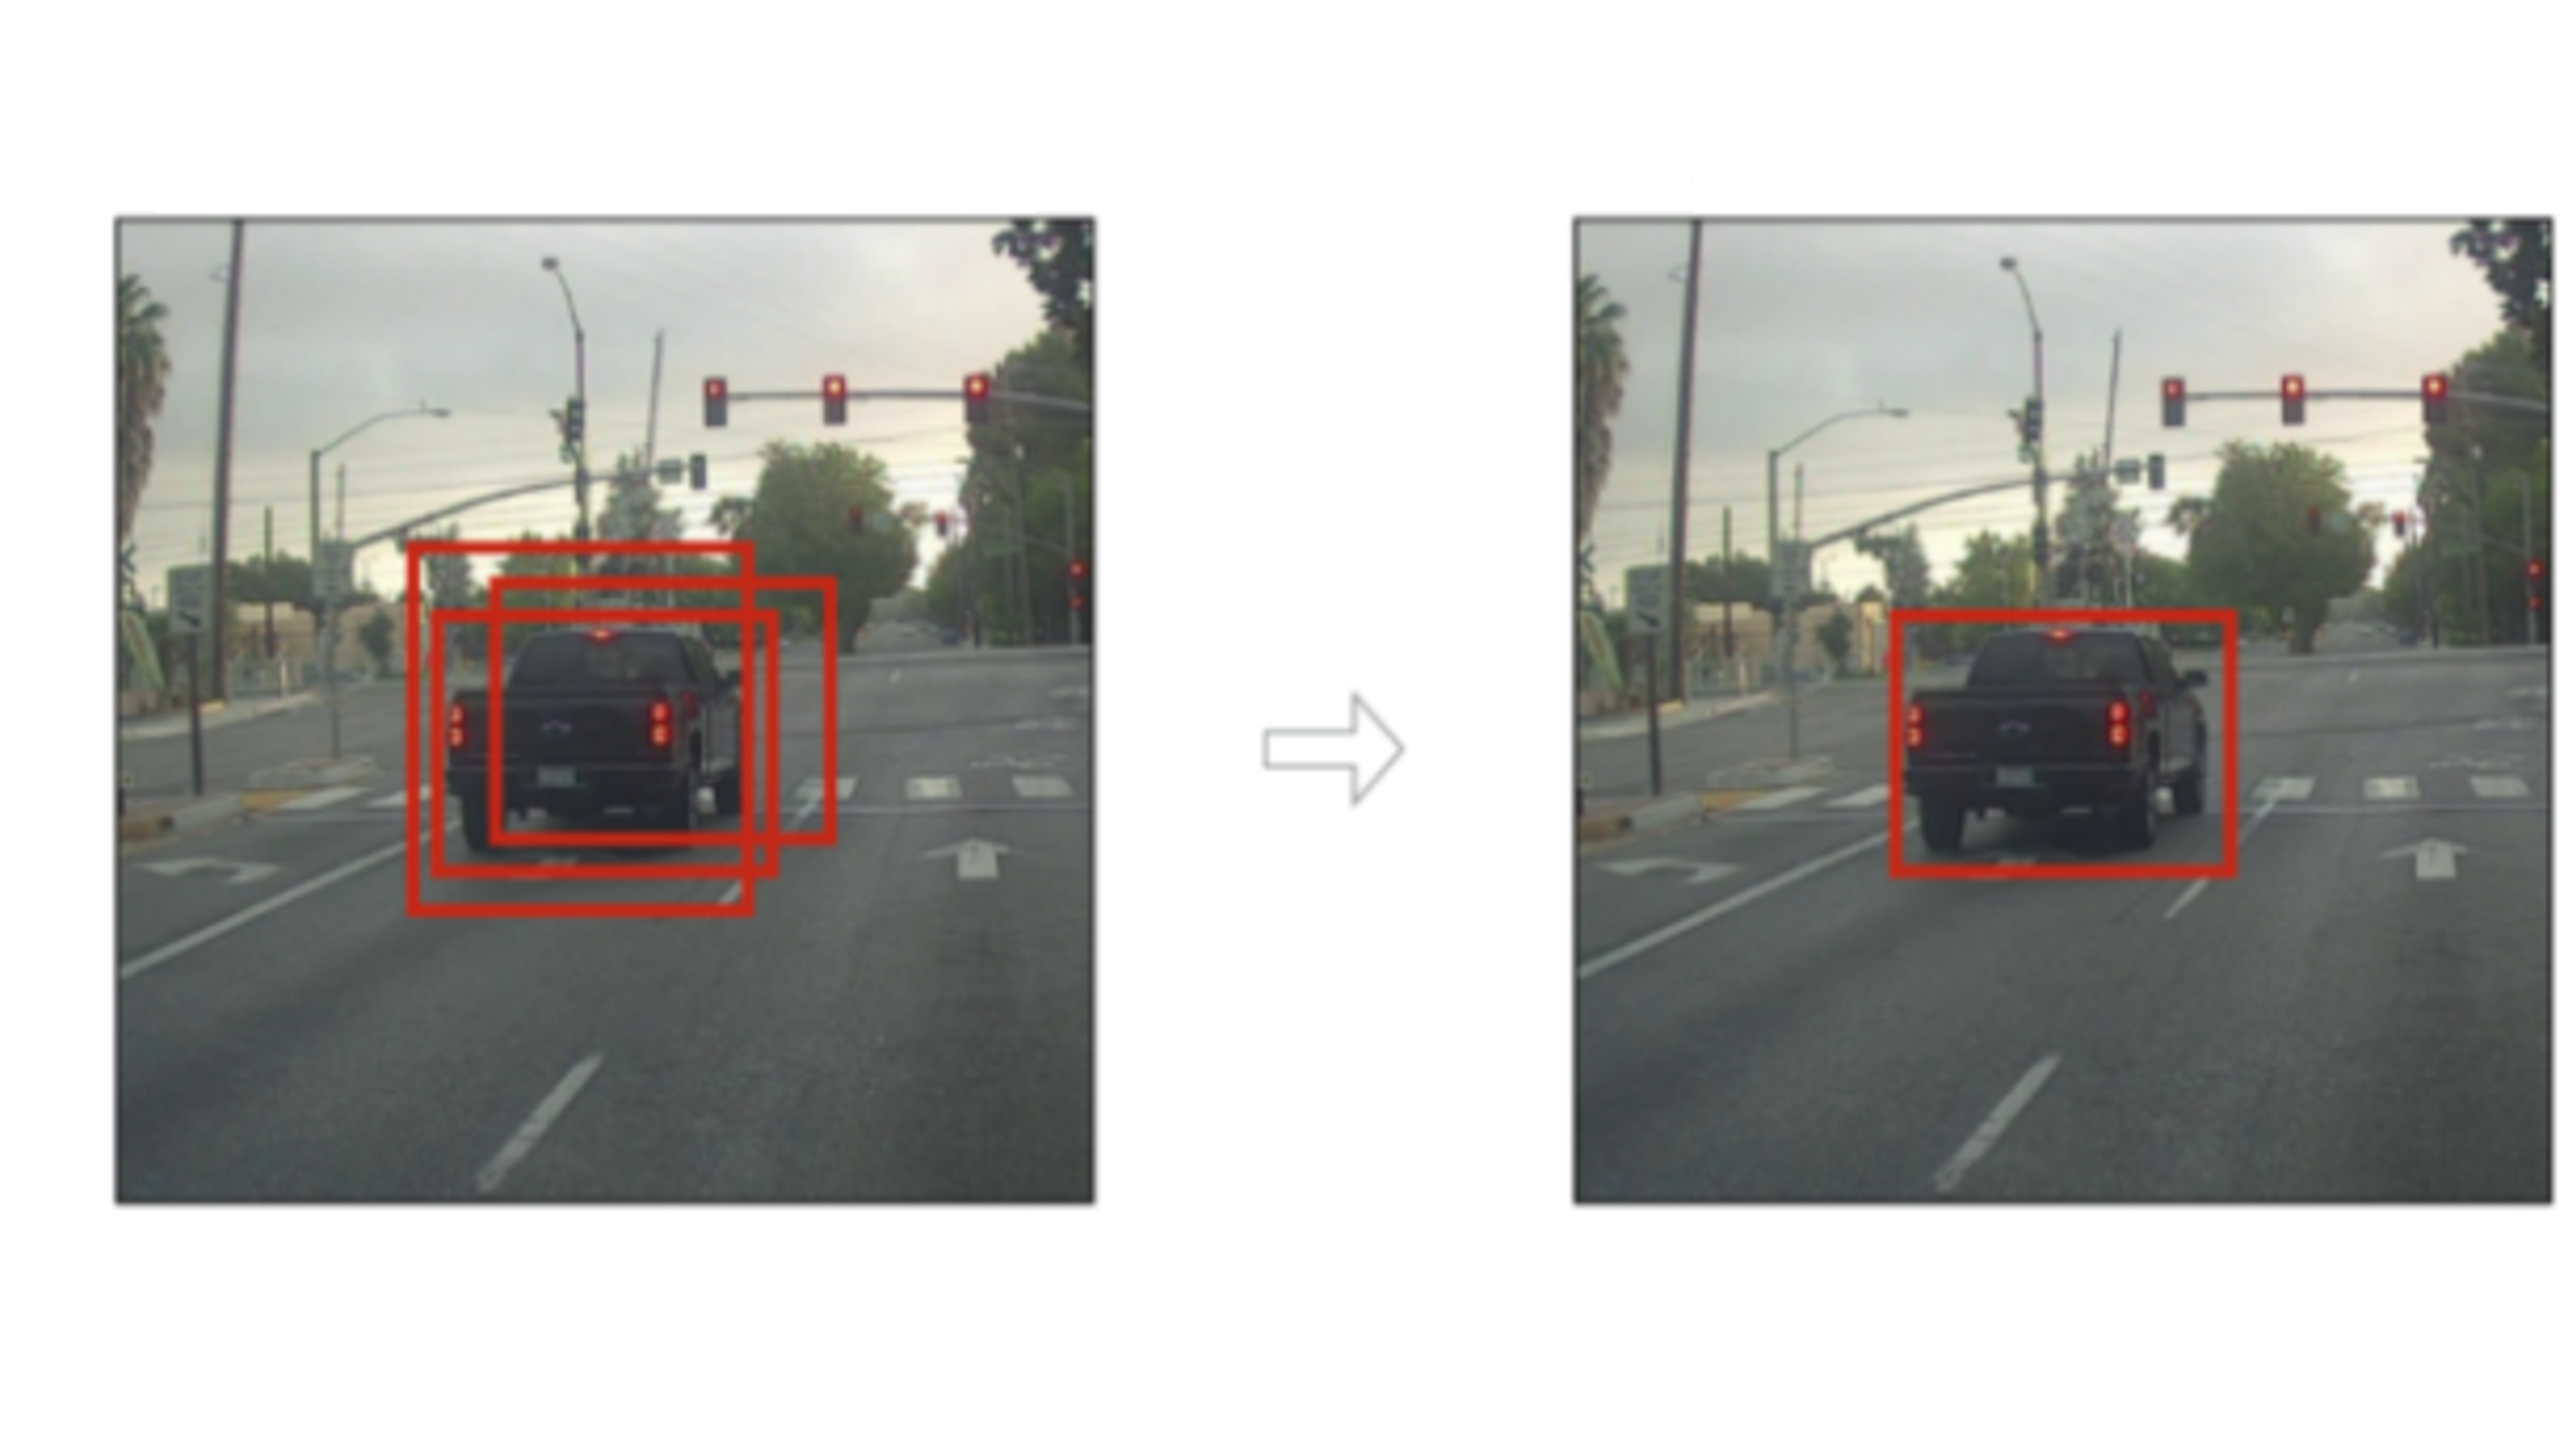
\includegraphics[width=\linewidth]{Images/interview.pdf}
\caption{(Left) The object detection system identifies many candidates for the location of the car. For each candidate, there is a score which measures how likely it is to find a car in that bounding box. You can see that there are multiple red boxes, where each box will have a score between 0-1. (Right) The final bounding box for the car.}
\label{interview}
\end{figure}

\begin{solution}
One process of selecting the final candidate amongst multiple candidate bounding boxes per object is Non-Max Suppression. The process prunes out bounding boxes of same object type which are close by a certain threshold and returns the best candidate.\\
The following steps are executed:\\
\textbf{Step 1:} Select the bounding box with the maximum score for one particular object type.\\
\textbf{Step 2:} Compare the IOU (Intersection Over Union) of this box with other boxes of same object type.\\
\textbf{Step 3:} Remove the boxes that have IOU over some threshold value.\\
\textbf{Step 4:} Select the next highest score bounding box and repeat steps 2-4 for remaining boxes.\\

\end{solution}


\end{document}